%!TEX root = main.tex

\subsection{\textbf{RQ1:} What processes do software developers utilize for merge conflicts?}\label{RQ1}

\boldif{Results from interviews indicated that a common model of operating with merge conflicts exists.}
To understand the processes of software developers when collaboratively working on code, we asked interview participants to describe their current processes for handling merge conflicts.

\boldif{\textit{Add anecdotal quotes and descriptions from interviews to highlight these observations.}}
Several participants describe using tools that alert them to potential or current merge conflicts, processes for analyzing and understanding conflicting code prior to implementing a resolution, and the use of tools and checklists for validating that their resolution worked.
In the interview, P3 describes this process as:
\begin{quoting}
\textit{``Part of my job on the integration team requires that I check for bad regressions. I use scripts to track patches as they're being backported, so I know when and where to look if [a patch] introduces a conflict. [\ldots] And once I've fixed [the conflict], I try to compare with the previous version to make sure [the code] works in a similar way.''}
\end{quoting}
As described above, the user becomes aware of a merge conflicting by using these scripts, plans to resolve them by maintaining information about the locations of things, and evaluates the resulting patches to verify that the conflict has been resolved.
\boldif{Provide descriptions that link the stages of Merge Conflict model to this quote. Use it to drive description of simplified model description paragraph}

\boldif{Based on these anecdotal observations, we construct an initial model of the processes that developers employ when working with merge conflicts, see Fig.~\ref{model}.}
Our interview results suggest that a model 

 we construct an initial model of the process developers experience between the introduction and resolution of merge conflicts.
Figure~\ref{model} provides an illustration of the model.
It consists of three phases: \emph{awareness, planning,} and \emph{evaluation.}

\boldif{Discuss the fact that no other studies have shown that a model exists for merge conflicts}

\begin{figure}[!htbp]
\centering
\fbox{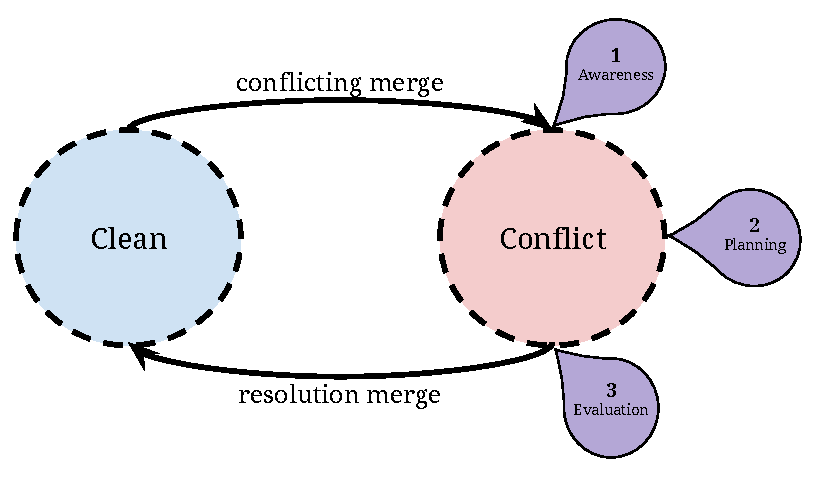
\includegraphics[width=0.98\textwidth,keepaspectratio]{imgs/MergeConflictModel}}
\caption{Model of Developer Processes for Merge Conflicts. Developers alternate between \textit{clean} and \textit{conflicting} states within their codebase. Developers maintain \textit{awareness}~(1) of conflicts within the codebase in different ways. Once aware, developers \textit{plan}~(2) a solution to fix the conflict. And finally, developers \textit{evaluate}~(3) the effectiveness of their deployed resolutions.}
\label{model}
\end{figure}

\boldif{Awareness is how developers become aware}
The \emph{awareness} phase consists of the actions developers take to become aware of merge conflicts.
This could be accidental, or passive, as the developer will become aware of a merge conflict when attempting to merge changes or perform a pull.
At the other end of the spectrum are developers who \emph{proactively} monitor for merge conflicts as they write code.
They are actively looking for changes that might be problematic, either manually or through the use of specialized tools.

\boldif{Planning is when developers plan their future actions}
Secondly, the \emph{planning} phase occurs after the developer has become aware that a conflict has occurred, and they are about to tackle the conflict.
This includes the decision of when they will try and resolve the conflict.
Some developers might try and resolve it immediately, while others might postpone the resolution.
Some might change their strategy depending on the conflict, incoming deadlines, etc.
This also includes other actions, such as if they are going to tackle the conflict alone, or collaborate with the person that made the other changes.

\boldif{Evaluation is how developers check that their solution is correct}
Finally, after the conflict has been resolved, developers enter in the \emph{evaluation} phase.
In this phase, the developer has to evaluate their resolution before considering the conflict as resolved.
This is to ensure the correctness of the resultant code.
Possible actions during this stage are compilation and building the product at one end.
Developer wanting more guarantees can go a step further and run the tests.
Finally, some groups might have policies such as code reviews that need to be performed on the merge conflict resolution.
 
\boldif{To explore and validate this model, we asked developers to reflect upon how they become aware of merge conflicts, how they plan for merge conflict resolutions, and how they evaluate their resolutions in the \textit{Processes Survey}~(S1).}
In order to explore and validate this model, and our assumptions, we conducted the \emph{Processes Survey}~(S1).
We plan on understanding how developers become aware of a merge conflicts (what steps they take, what tools they use, etc.)
We also want to investigate their strategies for dealing with merge conflicts and how they decide whether the resolution has addressed all of their concerns.

\boldif{We present the results to these research questions in Sections~\ref{RQ1a}, \ref{RQ1b}, and \ref{RQ1c}.}
Sections~\ref{RQ1a}, \ref{RQ1b}, and \ref{RQ1c} presents the results to these research questions.

\subsubsection{\textbf{RQ1a:} How do software developers become aware of merge conflicts?}\label{RQ1a}
\vspace*{-0.5\baselineskip}
\begin{quoting}
\textit{``It isn't that they cannot find the solution. It is that they cannot see the problem.'' -- G.K. Chesterton}
\end{quoting}
\vspace*{+0.3\baselineskip}

\begin{table}[!htbp]
\renewcommand{\arraystretch}{1.3}
\caption{Merge Awareness Toolsets (Top 10) from Processes Survey (S1)}
\label{s1_toolset}
\centering
\begin{tabularx}{\textwidth}{ll|c}
\toprule
  \parnoteclear % tabularx will otherwise add each note thrice
  Tool & Description & \# Participants (\%)\parnote{\textit{Processes Survey}~(S1) participants were allowed to provide multiple tools. Each entry represents the number (and percentage) of participants that responded with that particular tool. 57 out of 102 respondents (56\%) indicated the use of at least one merge awareness tool.}\\
\midrule
  Git & Version Control System & 32 (25.40\%)\\
  Email (unspecified) & Email Client or System & 7 (5.56\%)\\
  GitHub & Website & 7 (5.56\%)\\
  SVN & Version Control System & 4 (3.17\%)\\
  Visual Studio & IDE & 4 (3.17\%)\\
  PagerDuty & IT Incident Response Platform & 3 (2.38\%)\\
  GitLab & Website & 3 (2.38\%)\\
  Jenkins & Continuous Integration Platform & 3 (2.38\%)\\
  Team Foundation Server & Version Control System & 3 (2.38\%)\\
  VCS (unspecified) & Version Control System\hspace{1.9cm} & 3 (2.38\%)\\
\bottomrule
\end{tabularx}
\parnotes
\end{table}

\boldif{Developers use 2 methods for becoming aware of merge conflicts: proactive and reactive.}
From the Processes Survey (S1) we found that 32.26\% of participants do not actively monitor for merge conflicts during their development activities.
For the rest of the developers who answered with \emph{yes} or \emph{sometimes} (67.74\%), we identified 61 different tools in 126 instances.

\boldif{Reactive detection only notify developers that a merge conflict \emph{has happened}. Developers use it to minimize the size/complexity of the conflict, or it's impact on the team.}
Reactive monitoring for merge conflicts will only allow the developer to be notified after a merge conflict has occurred.
However, developers still use this process to manage or reduce the complexity of a conflict.
For the developers that answered that they monitor for merge conflicts (replied either \emph{yes} or \emph{sometimes}), we found that 73.68\% (42 out of 57 responses) described reactive processes.
For example, one developer said they use integration tools to detect merge problems before they advance to testing:
\begin{quotation}
	[\ldots] integration tests [\ldots] tell us if builds are breaking and we use those to locate merge conflicts. [\ldots] we use it to catch merge bugs before they go to smoke testing for release
\end{quotation}
Another developer mentioned that they try to solve merge conflicts early in order to minimize disruptions to the team:
\begin{quotation}
	We try to catch conflicts early so that fewer developers have to be involved in looking at broken code.
\end{quotation}

\boldif{Proactive monitoring allows devs to detect MC before they happen. However, it is more involved, as it requires a lot more manual effort from the developers.}
Proactive monitoring allows developers to preemptively catch merge conflicts before they happen.
Some developers mentioned they achieved this by manually tracking incoming changes:
\begin{quotation}
	I monitor commit logs before I begin merging branches so that I see any potentially overlapping code that will break the merge.
\end{quotation}
Other teams rely more on communication.
This can happen during regular team meetings, to make sure that everybody is aware of each other's tasks:
\begin{quotation}
	[\ldots] standups allow us to know where everyone is working that week.
\end{quotation}
Others will broadcast their changes in order to notify team members if they will make breaking changes:
\begin{quotation}
	[\ldots] send emails before making breaking changes to the API or related sub-modules.
\end{quotation}

\boldif{The tools that developers use allow for only a \emph{reactive} approach.}
Examining the tools used by respondents with reactive processes, we find that 87.72\% of our respondents use version control systems (Git, SVN, TFS, CVS), while 21.05\% use continuous integration systems (Jenkins, Travis CI, TeamCity).
Table~\ref{tab:tool-counts} presents the top 10 tools developers use when monitoring for merge conflicts.
The majority of the tools allow only a reactive approach to merge conflict monitoring.
It is worth noting that tools, such as those for Continuous Integration (CI) and developer notification systems (e.g. PagerDuty) are used only by developers relying on a \emph{reactive} strategy.

\boldif{Devs do not use existing workspace awareness tools that come from the acadmemia.}
When collaborating, developers generally rely on passive communication tools, like email, to coordinate.
Developers are currently not leveraging the functionalities provided by many research prototypes (e.g., Palant\'{i}r~\cite{palantir}, Crystal~\cite{Brun2011}) that are specifically designed to facilitate proactive conflict detection.

\begin{table}[hbt]
\caption{Top 10 tools used by developers when monitoring for merge conflicts. The counts are split into the two strategies: \emph{Reactive} and \emph{Proactive.}}
\label{tab:tool-counts}
\centering
\begin{tabular}{lccc}
\toprule
Tool & Proactive & Reactive & Total \\
\midrule
Git					& 10 & 30 & 40 \\
Email				& 2  & 4  & 6  \\
GitHub				& 2  & 5  & 7  \\
SVN					& 0  & 4  & 4  \\
Visual Studio		& 1  & 2  & 3  \\
PagerDuty 		    & 0  & 3  & 3  \\
GitLab				& 2  & 1  & 3  \\
Jenkins				& 0  & 3  & 3  \\
VCS (Unspecified)	& 2  & 2  & 4  \\
TFS					& 1  & 1  & 2  \\
\bottomrule
\end{tabular}	

\end{table}

\begin{comment}
We asked the Processes Survey (S1) participants to categorize and describe their monitoring processes: whether and how they monitor for merge conflicts, and how they determine the urgency of any merge conflicts that occur.
We found that 32.26\% of participants do not monitor for merge conflicts during their development sessions.
For the 67.74\% participants that indicate \textit{yes} or \textit{sometimes} to the question of monitoring for merge conflicts, we asked them to describe the processes and tools that they use for monitoring.

We identified 61 different tools from the 126 instances.
Some mentioned generic responses such as \textit{``email''}, for which we create a separate category.
Table~\ref{s1_toolset} lists the top 10 most common tools used by participants to monitor for merge conflicts.

In examining the list of these tools, we note that developers most often use version control systems (e.g. Git, SVN, TFS, and unspecified VCS) to handle tracking changes, and potentially identifying merge conflicts, within a codebase.
In this list, there is also one continuous integration (CI) platform (Jenkins), an IT incident response platform (PagerDuty), and two VCS-hosting websites (GitHub and GitLab).
This indicates that developers are currently relying on reactive tools that indicate the presence of merge conflicts after they have been introduced to a codebase.

We then evaluate responses for processes that are proactive or reactive in nature (using card sorting and negotiated agreement).
We find that 42 of 57 responses (73.68\%) described reactive processes of merge conflict monitoring; such as waiting for build systems notifications, examining commit logs, or checking code consistency during branch integration.

Examining the tools used by respondents with reactive processes, we find that 64.28\% of our respondents use version control systems (Git, SVN, TFS, CVS), while 29.19\% use continuous integration systems (Jenkins, Travis CI, TeamCity).
We find that developers are currently not leveraging the functionalities provided by many research prototypes (e.g., Palant\'{i}r~\cite{palantir}, Crystal~\cite{Brun2011}) that are specifically designed to facilitate proactive conflict detection.

\begin{table}[!htbp]
\renewcommand{\arraystretch}{1.2}
\caption{Factors for Determining the Urgency of a Merge Conflict from Processes Survey (S1)}
\label{s1_conflict_urgency}
\centering
\begin{tabularx}{\textwidth}{c | l | c | r}
\toprule
  \parnoteclear % tabularx will otherwise add each note thrice
  Factor & Description & \# Participants\parnote{Each entry represents the number (and percentage) of participants that indicated that particular factor was relevant. 72 out of 102 respondents (71\%) provided their factors.} & Percentage (\%)\\
\midrule
  F1 & No systematic factors & 22 & 30.56\% \\
  F2 & External dependencies & 17 & 23.61\% \\
  F3 & Code under conflict & 17 & 23.61\% \\
  F4 & Project structure & 16 & 22.22\% \\
\bottomrule
\end{tabularx}
\parnotes
\end{table}

In addition, we identified \textbf{X} distinct categories of processes that developers use to monitor for merge conflicts (see Table~\ref{s1_monitoring_processes}).
\boldif{Provide further discussion on the results of Q7 analysis; analysis between Caius and Nick still needed to group the processes into groups}
\boldif{Provide results and discussion for Q8; factors for determining urgency of a merge conflict.}

\end{comment}

\subsubsection{\textbf{RQ1b:} How do software developers plan for merge conflict resolutions?}\label{RQ1b}
\vspace*{-0.5\baselineskip}
\begin{quoting}
\textit{``If you are unable to understand the cause of a problem, it is impossible to solve it.'' –- Naoto Kan}
\end{quoting}
\vspace*{+0.3\baselineskip}

\boldif{Developers use different strategies for dealing with MC}
When encountering a merge conflict, developers have different strategies at their disposal.
They can either; (a) defer the merge conflict for a later date or; (b) try and solve the conflict.
In our Processes Survey (S1) we tried to get an understanding of these strategies and when developers use them.

\boldif{The first option is that they might defer the MC, for a later time}
The easiest option when encountering a merge conflict is to simply not deal with it.
Indeed, we found that 56.18\% of participants have deferred at least once when responding to a merge conflict.
The reasons for deferring are varied and include the \textit{complexity of the conflicting code} (D1), the \textit{number of conflicting code locations} (D2), and the \textit{ownership of the conflicting code} (D3) (Table~\ref{s1_deferring_response}).
One of the participants succinctly describes how they consider the \emph{ownership of the conflicting code} when deciding when to defer as:
\begin{quotation}
	Code is mine? I fix it. Code is others? I submit PR or bug reports.
\end{quotation}
This indicated that the deferral is not always temporal, but sometimes developers will defer to other team members.



\begin{table}[!htbp]
\renewcommand{\arraystretch}{1.2}
\caption{Factors in Deferring Responses to Merge Conflicts from Processes Survey (S1)}
\label{s1_deferring_response}
\centering
\begin{tabularx}{\textwidth}{>{\rowmac}c | >{\rowmac}l | >{\rowmac}c | >{\rowmac}r <{\clearrow}}
\toprule
  \parnoteclear % tabularx will otherwise add each note thrice
  Factor & Description & \# Selections\parnote{\textit{Processes Survey}~(S1) respondents were allowed to select multiple factors. 44 out of 102 respondents (43\%) selected more than one factor.} & Percentage (\%)\textsuperscript{i} \\
\midrule
  D1 & Complexity of the conflicting code & 36 & 25.00\% \\
  D2 & Number of conflicting code locations & 32 & 22.22\% \\
  D3 & Ownership of the conflicting code & 25 & 17.36\% \\
  D4 & Size of the conflicting code & 20 & 13.89\% \\
  D5 & Approaching deadlines & 13 & 9.03\% \\
  D6 & Work schedule constraints & 2 & 1.39\% \\
  D7 & Other\hspace{4.6cm} & 7 & 4.86\% \\
\bottomrule
\end{tabularx}
\parnotes
\end{table}

\boldif{Deferring can have bad consequences, including increased complexity and delaying features.}
Deferring the resolution does not come without it's price.
Figure~\ref{fig:effects-deferral} shows the top effects of a deferral.
The most common effect was that developers have had to stop the development (\emph{Stop the Presses,} 15 responses) in order to resolve the conflicts.
The second most common effect is the increased complexity of the conflicts, as it was reported by 9 of our participants.
One participant noted that:
\begin{quotation}
	Deferring a merge conflict simply kicks the can down the road (or off a cliff). Typically resolving the conflict only gets more difficult as time passes.
\end{quotation}
A respondent even hinted that the complexity increase can be quite severe, of orders of magnitude:
\begin{quotation}
	Untangling takes days instead of minutes when it gets too out of hand.
\end{quotation}
In some cases, features had to be removed from releases, in order for the integration problems to be successfully resolved:
\begin{quotation}
	We have had several releases come up short in new features because they got delayed by integration problems.
\end{quotation}

\boldif{However, some effect can be severe, including impact to customers, or having to reimplement features}.
In one extreme case, a participant reported that the effects of a unresolved merge conflicts affected production software, which resulted in downtime of the product, as it broke functionality:
\begin{quotation}
	Broke the app for customers until we could get a patch pushed [\ldots].
\end{quotation}
Finally, the merge conflicts can get too severe, and developers have to resort to the \emph{Nuclear Option}, where they scrap their changes and reimplement them:
\begin{quotation}
	Uh.... KABOOM! More changes came in and everything piled up. Nothing to do but wipe it all back to clean and start trying to piece things back together.
\end{quotation}

\begin{figure}
	\centering
	\fbox{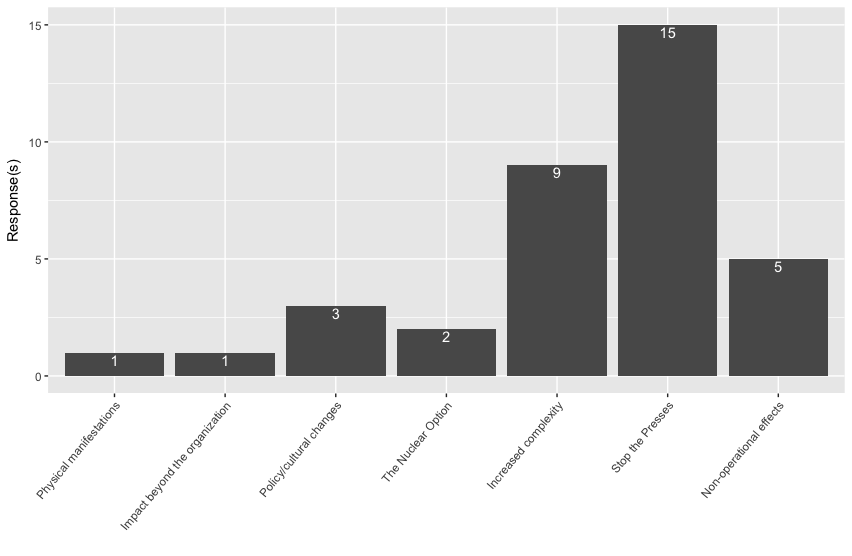
\includegraphics[width=0.9\textwidth,keepaspectratio]{EffectsDeferral.png}}
	\caption{The effects of deferring a merge conflicts. It the majority of cases, the developers end up having to stop the development in order to resolve the problems.}
	\label{fig:effects-deferral}
\end{figure}

\boldif{If they have not deferred, they need to understand the (changes in the) conflict}
Other than deferring, the other remaining option for developers is to resolve the conflict.
They primarily approach merge conflicts by \textit{examining the conflict} (U1), \textit{analyzing or manipulating the code} (U2), or \textit{examining the code} (U3) (see Table~\ref{s1_understanding_code}).

\begin{table}[!htbp]
\renewcommand{\arraystretch}{1.2}
\caption{Initial Strategies for Understanding Conflicting Code from Processes Survey (S1)}
\label{s1_understanding_code}
\centering
\begin{tabularx}{\textwidth}{>{\rowmac}c | >{\rowmac}l | >{\rowmac}c | >{\rowmac}r <{\clearrow}}
\toprule
  \parnoteclear % tabularx will otherwise add each note thrice
  Strategy & Description & \# Participants\parnote{79 out of 102 respondents (77\%) provided a description of their initial strategy.} & Percentage (\%)\textsuperscript{i} \\
\midrule
  U1 & Examining the conflict & 26 & 32.91\% \\
  U2 & Analysis/manipulation of the code & 19 & 24.05\% \\
  U3 & Examining the code & 18 & 22.79\% \\
  U4 & Focus on design concerns & 8 & 10.13\% \\
  U5 & Examine project organization & 6 & 7.60\% \\
  U6 & No strategy\hspace{3.5cm} & 2 & 2.53\% \\
\bottomrule
\end{tabularx}
\parnotes
\end{table}
\vspace{0.8em}

\boldif{The most common strategies for understanding the conflict are examining the conflict and analysis/manipulation of the code.}
One participant described their strategy of examining the conflict as:
\begin{quotation}
	Reviewing the most recent commits (comments and code) to see whether its a shallow conflict or not.
\end{quotation}
	Another participant indicated their strategy of analyzing the code involves:
\begin{quotation}
[\ldots] determining if the merge conflict involves important functionality; stepping through with a debugger helps.
\end{quotation}
Overall, we find that developers initially focus on the code involved in the merge conflict or information related to the conflict itself.

\boldif{Surprisingly, some developers do not have a strategy for MCR}
Surprisingly, we found that two of our participants (2.53\% of respondents) indicated that they \textit{``don't have a strategy''} or \textit{``mostly try to fix it as soon as possible.''}
The existence of this \textit{no strategy} approach is anecdotal, but curious, since we assume that developers are rational actors seeking to organize themselves in ways that increase the likelihood of successful outcomes.
And yet this strategy appears to go counter to that notion.

\begin{figure}[!htbp]
\centering
\fbox{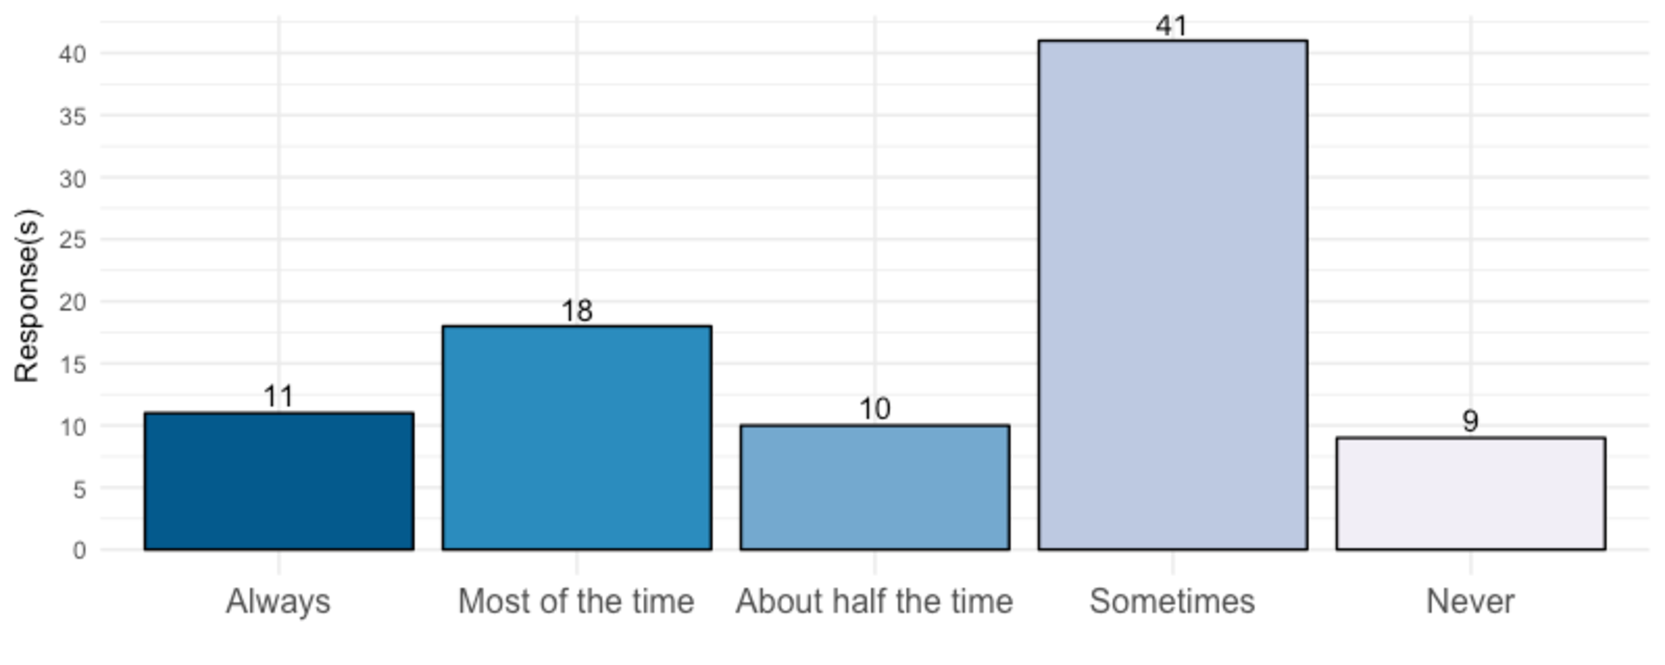
\includegraphics[width=0.98\textwidth,keepaspectratio]{imgs/CodeOwnershipFactor}}
\caption{Degree of Code Ownership as a Factor in Merge Conflict Strategies. Scale: 1 is \textit{Always} and 5 is \textit{Never}. 89 out of 102 respondents (87.26\%) provided a response to this question in the \textit{Processes Survey}~(S1).}
\label{fig:code-ownership-resolution}
\end{figure}

\boldif{The role of code ownership in the resolution strategy.}
Finally, we found that, on average, participants indicate that code ownership factors \textit{about half the time} in their strategy of code ownership (mean: 3.21 on a 5-point Likert-type scale).
This is consistent with their responses for their criteria for deferring a resolution, where it is the third most common factor in their decision. 
Only 10.11\% of participants indicated that code ownership \textit{never} factors into their resolution strategy (see Figure~\ref{fig:code-ownership-resolution}).

\begin{comment}

Software developers adopt strategies for increasing their own efficiency and productivity.
We asked Process Survey (S1) participants a series of questions relating to their strategies for gaining understanding about a merge conflict, prioritizing merge conflict resolutions, and deferring resolutions when necessary.

\subsubsection{Initial Strategies for Understanding Conflicting Code}

We asked participants to describe their initial strategies for understanding conflicting code involved in a merge conflict.
We find that developers primarily approach merge conflicts by \textit{examining the conflict} (U1), \textit{analyzing or manipulating the code} (U2), or \textit{examining the code} (U3) (see Table~\ref{s1_understanding_code}).

One participant described their strategy of examining the conflict as:
\begin{quoting}
\textit{``Reviewing the most recent commits (comments and code) to see whether its a shallow conflict or not.''}
\end{quoting}
Another participant indicated their strategy of analyzing the code involves:
\begin{quoting}
\textit{``[\ldots] determining if the merge conflict involves important functionality; stepping through with a debugger helps.''}
\end{quoting}
Overall, we find that developers initially focus on the code involved in the merge conflict or information related to the conflict itself.
This illustrates the importance of code metrics and tool support for developers looking to gain understanding about a merge conflict when planning for a resolution.

Surprisingly, we found that two of our participants (2.53\% of respondents) indicated that they \textit{``don't have a strategy''} or \textit{``mostly try to fix it as soon as possible.''}
The existence of this \textit{no strategy} approach is anecdotal, but curious, since we assume that developers are rational actors seeking to organize themselves in ways that increase the likelihood of successful outcomes.
And yet this strategy appears to go counter to that notion.

\begin{table}[!htbp]
\renewcommand{\arraystretch}{1.2}
\caption{Initial Strategies for Understanding Conflicting Code from Processes Survey (S1)}
\label{s1_understanding_code}
\centering
\begin{tabularx}{\textwidth}{>{\rowmac}c | >{\rowmac}l | >{\rowmac}c | >{\rowmac}r <{\clearrow}}
\toprule
  \parnoteclear % tabularx will otherwise add each note thrice
  Category & Description & \# Participants\parnote{79 out of 102 respondents (77\%) provided a description of their initial strategy.} & Percentage (\%)\textsuperscript{i} \\
\midrule
  U1 & Examining the conflict & 26 & 32.91\% \\
  U2 & Analysis/manipulation of the code & 19 & 24.05\% \\
  U3 & Examining the code & 18 & 22.79\% \\
  U4 & Focus on design concerns & 8 & 10.13\% \\
  U5 & Examine project organization & 6 & 7.60\% \\
  U6 & No strategy & 2 & 2.53\% \\
\bottomrule
\end{tabularx}
\parnotes
\end{table}
\vspace{0.8em}

\subsubsection{Deferring Responses to Merge Conflicts}

We also found that 56.18\% of participants have deferred responding to a merge conflict.
To understand the rationale behind deferring, we asked the participants to select the factors they consider when trying to determine whether they will defer their response to a merge conflict.

\begin{table}[!htbp]
\renewcommand{\arraystretch}{1.2}
\caption{Factors in Deferring Responses to Merge Conflicts from Processes Survey (S1)}
\label{s1_deferring_response}
\centering
\begin{tabularx}{\textwidth}{>{\rowmac}c | >{\rowmac}l | >{\rowmac}c | >{\rowmac}r <{\clearrow}}
\toprule
  \parnoteclear % tabularx will otherwise add each note thrice
  Factor & Description & \# Participants\parnote{\textit{Processes Survey}~(S1) respondents were allowed to select multiple factors. 44 out of 102 respondents (43\%) selected more than one factor.} & Percentage (\%)\textsuperscript{i} \\
\midrule
  D1 & Complexity of the conflicting code & 36 & 25.00\% \\
  D2 & Number of conflicting code locations & 32 & 22.22\% \\
  D3 & Ownership of the conflicting code & 25 & 17.36\% \\
  D4 & Size of the conflicting code & 20 & 13.89\% \\
  D5 & Approaching deadlines & 13 & 9.03\% \\
  D6 & Work schedule constraints & 2 & 1.39\% \\
  D7 & Other & 7 & 4.86\% \\
\bottomrule
\end{tabularx}
\parnotes
\end{table}

The top three reasons that developers defer responding to a merge conflict are: \textit{complexity of the conflicting code} (D1), \textit{number of conflicting code locations} (D2), and \textit{ownership of the conflicting code} (D3) (see Table~\ref{s1_deferring_response}).
Previous studies have shown that increases in the perception of \textit{complexity of conflicting code} are associated with increases in the perception of merge conflict difficulties~\cite{mckee2017software}.
If developers are deferring code that they perceive as complex, then some of the perceived difficulties might arise from developers delaying resolutions and being forced to untangle additional code changes made on top of the conflicting code.

As the third most selected choice, \textit{ownership of the conflicting code} (D3) indicates that group dynamics play a role in merge conflicts.
One of the participants succinctly describes this factor in their response:
\begin{quoting}
\textit{``Code is mine? I fix it. Code is others? I submit PR or bug reports.''}
\end{quoting}

\begin{figure}[!htbp]
\centering
\fbox{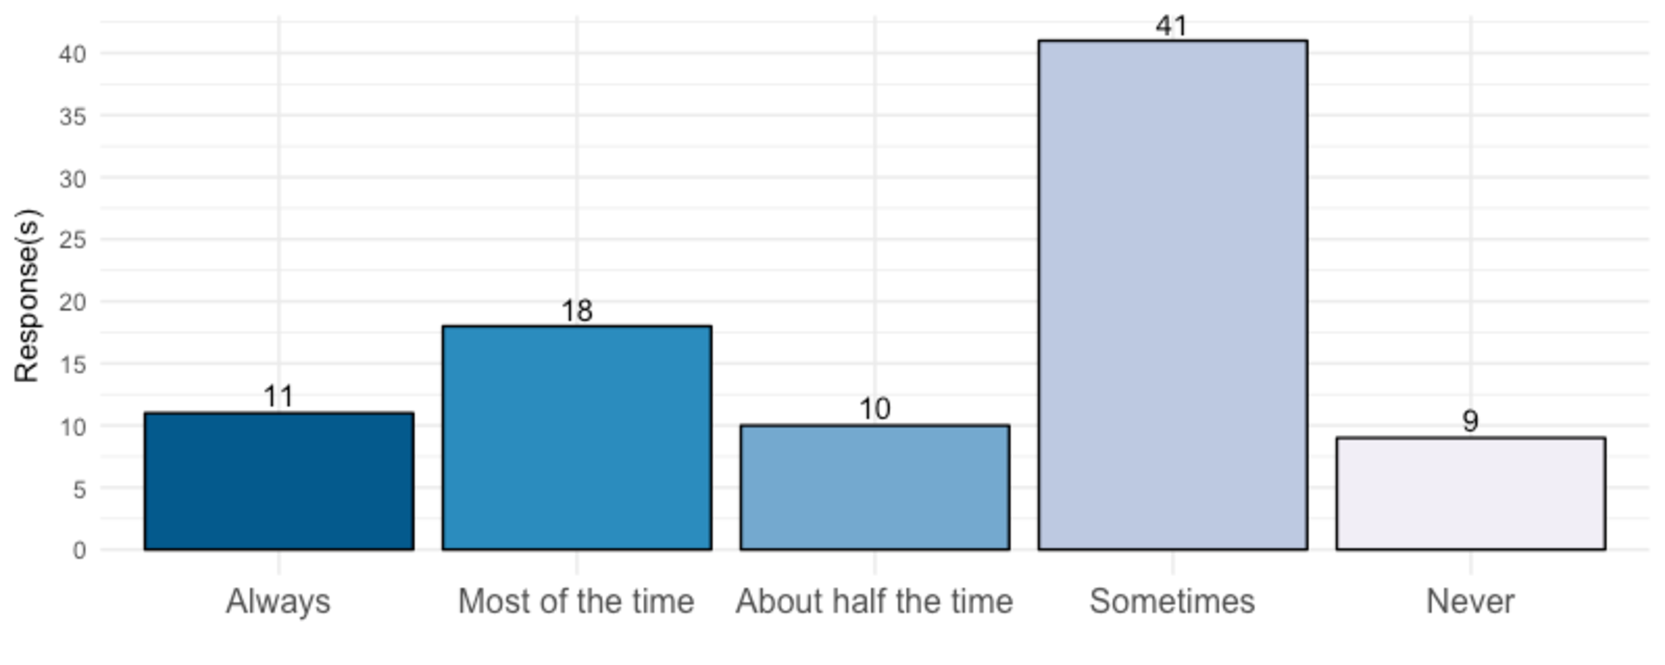
\includegraphics[width=0.98\textwidth,keepaspectratio]{imgs/CodeOwnershipFactor}}
\caption{Degree of Code Ownership as a Factor in Merge Conflict Strategies. Scale: 1 is \textit{Always} and 5 is \textit{Never}. 89 out of 102 respondents (87.26\%) provided a response to this question on the \textit{Processes Survey}~(S1).}
\label{model}
\end{figure}

As an additional question to explore this factor, we asked participants how often \textit{code ownership} factored into their merge conflict resolution strategy.
We found that on average participants indicate that it factors in \textit{about half the time} (mean: 3.21 on a 5-point Likert-type scale).
Only 10.11\% of participants indicated that code ownership \textit{never} factors into their resolution strategy (see Figure~\ref{s1_conflict_urgency}).
\end{comment}

\subsubsection{\textbf{RQ1c:} How do software developers evaluate merge conflict resolutions?}\label{RQ1c}

\vspace*{-0.5\baselineskip}
\begin{quoting}
\textit{``We fail more often because we solve the wrong problem than because we get the wrong solution to the right problem.'' –- Russell L. Ackoff}
\end{quoting}
\vspace*{+0.3\baselineskip}

After implementing a merge conflict resolution, software developers must evaluate whether their resolution has returned the codebase to a clean state.
However, it is unclear what conditions are considered by developers to be the benchmark for successful merge conflict resolutions.

\vspace*{0.8\baselineskip}
\noindent\textit{Success Conditions for Merge Conflict Resolutions}
\vspace*{0.5\baselineskip}

To understand which conditions of merge conflict resolutions might be the benchmarks, we examined the results of the \textit{Exploratory Interview} and found six common conditions that developers described as being important to their resolution strategies.
We asked developers in the \textit{Processes Survey}~(S1) to select all conditions that they would consider to be a successful merge conflict resolution from this list of six conditions.
We included an open-ended \textit{other} option to allow for additional conditions to surface, but only two developers selected that condition (indicating \textit{performance tests showing similar performance} and \textit{client approval}).
We received 324 selections from 89 respondents and present the aggregated results in Table~\ref{conditionsSuccess}.

\begin{table}[!htbp]
%\renewcommand{\arraystretch}{1.3}
\caption{Conditions of Successful Merge Conflict Resolutions from Processes Survey (S1)\textsuperscript{i}}
\label{conditionsSuccess}
\centering
\begin{tabularx}{\textwidth}{@{}lr|*{7}{C}c@{}}
\toprule
\addlinespace[4.9em]
	\multicolumn{2}{@{}l}{\noindent Condition}
	& \begin{rotate}{30} All tests pass \end{rotate}
	& \begin{rotate}{30} Code compiles \end{rotate}
	& \begin{rotate}{30} VCS warnings gone \end{rotate}
	& \begin{rotate}{30} Merged to production \end{rotate}
	& \begin{rotate}{30} Code looks correct \end{rotate}
	& \begin{rotate}{30} Code reviewed \end{rotate}
	& \begin{rotate}{30} Other \end{rotate} \\
\midrule
	C1 & All tests pass & 67 & & & & & & \\
	C2 & Code compiles & 50 & 67 & & & & & \\
	C3 & VCS warnings gone & 38 & 42 & 51 & & & & \\
	C4 & Merged to production & 27 & 27 & 26 & 33 & & & \\
	C5 & Code looks correct & 50 & 54 & 41 & 27 & 66 & & \\
	C6 & Code reviewed & 32 & 31 & 25 & 19 & 27 & 38 & \\
	C7 & Other & 2 & 2 & 0 & 0 & 2 & 0 & 2 \\
\bottomrule
    \multicolumn{9}{c}{\noindent\parbox[t]{11.7cm}{\vspace{0.4em}\textsuperscript{i}\hspace{0.2em}\textit{Processes Survey}~(S1) respondents were allowed to select multiple conditions. Each entry represents the number of respondents that selected both of the conditions indicated for the column and row. 68 out of 102 respondents (67\%) selected three or more conditions.}} \\
\end{tabularx}
\end{table}

The most commonly selected conditions that signify a successful merge conflict resolution were when \textit{all tests pass} (C1), \textit{code successfully compiles} (C2), and \textit{code looks correct (i.e. visual test passes)} (C3).
The use of testing (C1) as both functionality and code quality assurance measures are well-known~\cite{beizer1984software}\cite{tian2005software}, and have been fundamental to  development processes such as test-driven development for several years~\cite{beck2003test}.
Similarly, the use of compilers to validate code (C2) as being executable and in good-working order will be familiar to any developer using an interpreted programming language.

The use of visual inspection as a measure of successful merge conflict resolutions is surprising, given that \textit{complexity of conflicting lines of code} is the highest rate factor for impacting merge conflict difficulty~\cite{mckee2017software}.
Inspecting code requires time and expertise in the area of conflicting code.
The survey respondents that selected \textit{code looks correct (i.e. visual test passes)} had a mean of 9.2 years of programming experience, which is only slightly higher than the overall mean of 9.0 years of programming experience.

Looking at the combination of \textit{code looks correct (i.e. visual test passes} with the other conditions, we find that 54 respondents also selected \textit{all tests pass} (52.9\%).
As the most common pairing of selected conditions on the \textit{Processes Survey}~(S1), we conclude that although developers rely upon their expertise to visually inspect a merge conflict resolution, they also verifying their observations through testing.

\vspace*{0.8\baselineskip}
\noindent\textit{Merge Conflict Resolution Toolsets}
\vspace*{0.5\baselineskip}

As conditions such as testing and compilation are used to gauge the success of a merge conflict resolution, it is also important to understand the tools that developers are relying upon for evaluating resolutions.
Using the \textit{Exploratory Interviews} responses to guide us, we found five categories of software development tools that developers discuss in relation to merge conflicts.
We then asked \textit{Processes Survey}~(S1) participants to select the categories of tools that they use to assist in evaluating whether their conflict resolutions have met the conditions for success.
We received 204 selections from 89 respondents and present the aggregated results in Figure~\ref{fig:resolution-evaluation-tools}.

\begin{figure}
	\centering
	\fbox{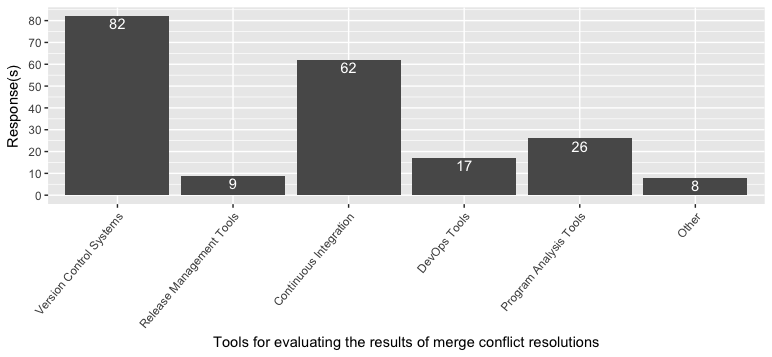
\includegraphics[width=0.95\textwidth,keepaspectratio]{ResolutionEvaluationTools.png}}
	\caption{Tools for evaluating the results of merge conflict resolutions}
	\label{fig:resolution-evaluation-tools}
\end{figure}

By far the most selected tools were \textit{version control systems} (VCS) and \textit{continuous integration} (CI) platforms, with 82 (40.2\%) and 62 (30.4\%) respectively.
All other tool categories combined had a mean of only 15 selections and represent only 29.4\% of response selections.

The use of \textit{continuous integration} requires that tests be written and maintained, and can only provide meaningful information when code is compilable.
We note that this result is in line with the inclusion of \textit{all tests passing} (C1) and \textit{code successfully compiles} (C2) as the most common conditions for a successful merge conflict resolution.
However, the availability of tools for evaluating merge conflict resolutions might be constraining the conditions that developers are willing and able to use.
Further research is needed to determine whether additional metrics and conditions for success are needed to more effectively evaluate merge conflict resolutions.

\vspace*{0.8\baselineskip}
\noindent\textit{Backup Strategies}
\vspace*{0.5\baselineskip}

Merge conflict resolutions are not always successful.
When they fail, developers have to alter their resolutions and potentially switch strategies in order to successfully resolve the conflict.

To understand the prevalence of failed conflict resolutions, we asked \textit{Processes Survey} (S1) participants to indicate the frequency in which their first attempt at resolving a merge conflict fails.
Figure~\ref{fig:first-attempt-failure} illustrates the resulting distribution.
On the 5-point Likert-type scale, where 1 is \textit{very frequently} and 5 is \textit{very infrequently}), the mean response was 3.49 (std. dev. = 1.11, variance = 1.24).
This corresponds to \textit{somewhat infrequently} being the average response, which suggests that first attempts typically succeed.
However, this does show that for 78.7\% (70 out of 89) of participants occasionally have to make another attempt at resolving a merge conflict.

\begin{figure}
	\centering
	\fbox{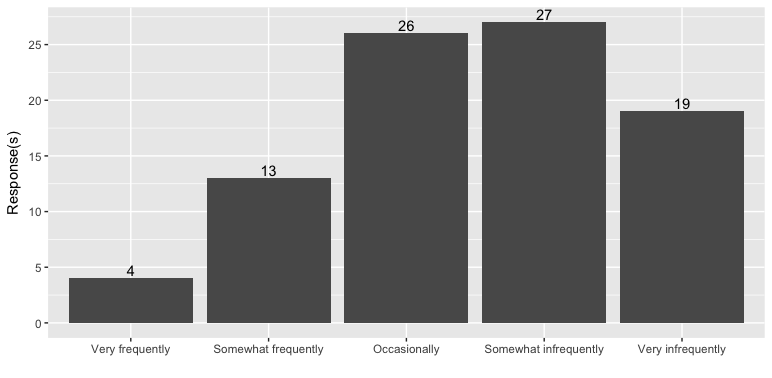
\includegraphics[width=0.95\textwidth,keepaspectratio]{FirstAttemptFailure.png}}
	\caption{Frequency of first attempt failures of merge conflict resolutions}
	\label{fig:first-attempt-failure}
\end{figure}

Further, we asked survey participants to describe their backup strategies for when their first attempt at resolving a merge conflict fails.
We received 75 responses and present the aggregate results in Figure~\ref{fig:backup-strategies}.
Developers use a variety of strategies for resolving merge conflicts, and their backup strategies include \textit{take it offline} (S1), \textit{collaborating} (S2), \textit{try again} (S3), \textit{redoing changes} (S4), and \textit{no backup strategy} (S5).
Since \textit{no backup strategy} (S5) is not a strategy in and of itself, we focus these results on strategies S1-S4 instead.

The \textit{take it offline} (S1) strategy involves moving conflicting code away from shared branches or code repositories, and working locally to resolve the conflict without disrupting other developers.
The antithesis of this strategy is \textit{collaborating} (S2), where developers seek out other developers that are more knowledgeable about the area of conflicting code.
The S1 and S2 strategies contrast each other, and show that developers reserve more costly strategies (in terms of time, effort, and coordination) as backups.

Additionally, we find that developers also simply \textit{try again} (S3) to merge the same code together and hope that their tools are able to succeed with a second attempt.
Developers also resort to \textit{redoing changes} (S4), by way of reverting and manually recreating the changes found in conflicting commits, when their initial attempts fail.
The S3 and S4 strategies appear to cement the extremes of the cost spectrum of backup strategies for resolving merge conflicts.
Where simply retrying the same merge (S3) requires vary little additional work, the process of redoing changes (S4) is a duplication of previous efforts and costly on developer's time.

\begin{figure}
	\centering
	\fbox{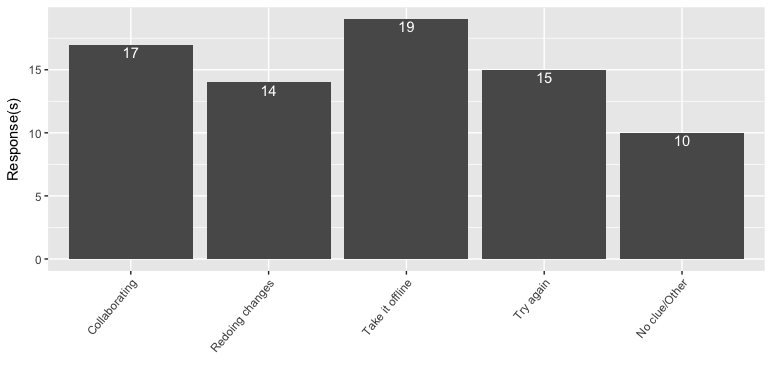
\includegraphics[width=0.95\textwidth,keepaspectratio]{BackupStrategies.png}}
	\caption{Backup strategies of developers for merge conflict resolutions.}
	\label{fig:backup-strategies}
\end{figure}
